\documentclass[twocolumn, a4paper]{UECIEresume}

\usepackage[dvipdfmx]{graphicx}
\usepackage{otf} % ハシゴダカは\UTF{9AD9}
\usepackage{algorithm}
\usepackage{algorithmic}
\usepackage{graphicx}
\usepackage{amsmath}
\usepackage{txfonts}

\title{個体間距離を考慮した複数解探索型Bat Algorithm}
\date{平成 30 年 9 月 24 日}
\affiliation{情報学専攻 メディア情報学 プログラム}
\supervisor{\UTF{9AD9}玉 圭樹 教授, 佐藤 寛之 准教授}
\studentid{1730022}
\author{岩瀬 拓哉}
% \headtitle{平成 yy 年度 総合情報学科 卒業論文中間発表}
%\headtitle{平成 yy 年度 総合情報学科 卒業論文発表}
\headtitle{平成 30 年度 情報学専攻 修士論文中間発表}
%\headtitle{平成 yy 年度 総合情報学科 修士論文発表}

\begin{document}
\maketitle

\section{はじめに}
多峰性最適化問題における,従来の多点探索アルゴリズムは一つの最適解に収束する傾向にあるが,環境が変化する実問題への適用を考慮した時に複数の最適解及び局所解を探索し,保持しておくことは非常に重要な意味を持つ.本研究では,大域探索と局所探索のバランスの調整に優れたBat Algorithmを用い,個体が同じ解に収束しないよう分散させるNiche Radiusによる複数解探索可能なアルゴリズムを構築する.

\section{従来手法}
\subsection{Bat Algorithm}
Bat Algorithm(BA)は群知能アルゴリズムの一つで,対象物までの方向や距離を知るコウモリの特性(エコロケーション)を利用して周囲の状況を認知し,大域的な探索が進むにつれて探索速度を徐々に調節することが可能なアルゴリズムである\cite{BA}.BAにおいて,コウモリは自らの発する超音波の周波数を持ち,その周波数を調整するためのパラメータとしてラウドネス${A}$を用いる.
% ラウドネス${A}$は,コウモリが対象物に近づくと値が減少し,移動距離も比例して短くなる.
コウモリの行動は以下3つの特徴で構成される.\\
i. 各コウモリは,自身が発する周波数${f_i}$の反響によって対象物との距離を知る.\\
ii. コウモリは位置${x_i}$において速度${v_i}$で,対象物に近い他のコウモリの方へランダムに移動する.\\
iii. コウモリが対象物に近づくにつれて,ラウドネス${A}$を減少させる.

\section{提案手法}

\subsection{Niche Radius based Bat Algorithm}
個体間同士の距離が近い場合に遠ざかる方向へ移動させる機構を持つNiche Radiusを用い,本研究では同じ解に個体が収束しないよう分散させ,複数解を探索可能なアルゴリズムを提案する.Niche Radius\cite{niche}は解空間のスケールと最適解数から算出した距離(NR)であり,式(\ref{eq:lambda}),(\ref{eq:NR})で表される.

\begin{equation}
\label{eq:lambda}
\lambda =\frac{1}{2} \sqrt{(x_{ub}-x_{lb})^2}
\end{equation}
\begin{equation}
\label{eq:NR}
NR=\frac{\lambda}{\sqrt[D]{q}}
\end{equation}
$x_{ub}$,${x_{lb}}$は解空間の上限と下限を示し,${D}$は次元数,$q$は最適解の数を表す.
% 各個体が持つNRより個体間同士の距離$d_i$が小さい場合のみ,個体から遠ざかる方向へ移動させる.
各個体の周波数${f_i}$,速度${v_i}$,位置${x_i}$は以下の式で定義し,更新される.

\begin{equation}
\label{eq:freq}
f_i=f_{min}+(f_{max}-f_{min}) \beta
\end{equation}
\begin{equation}
\label{eq:vi}
v_i^{t+1}=v_i^t+(x_i^t-x_{NR*}^t)*f_i
\end{equation}
\begin{equation}
\label{eq:xi}
x_i^{t+1}= \begin{cases}
x_i^t+v_i^{t+1} & (if \ d_i^t < NR) \\
x_i^t & (else)
\end{cases}
\end{equation}
各個体の周波数${f_i}$は個体の速度を制限するパラメータであり,$[0 \ 1]$の区間で表される.ここでは${f_{min}=0}$,${f_{max}=1}$として設定する.個体のNRより個体間距離${d_i}$が小さいとき,式(\ref{eq:vi})にてNR内の最良解${x_{NR*}}$から離れる方向へ速度${v_i}$より${x_i}$は移動する. \\
次に,NR内の最良解${x_{NR*}}$の周辺に新しい解${x_{loc}}$を生成する.生成式は次の通りである.
\begin{equation}
\label{eq:loc}
x_{loc}=x_{NR*} + \epsilon A_i^t
\end{equation}
パラメータ$\epsilon$は1 $\times$ d次元の配列で$[-NR \ NR]$区間のランダムな値が割り当てられる. \\
最後に,${x_i^{t+1}}$あるいは${x_{loc}}$での個体の評価値がパーソナルベストより良ければ更新され,ラウドネス$A$とその反射波であるパルスレート$r$も以下の式に基づいて更新される.
\begin{equation}
\label{eq:loud}
A_i^{t+1}= \alpha A_i^t
\end{equation}
\begin{equation}
\label{eq:pulse}
r_i^{t+1}=r_i^t[1-exp(- \gamma t)]
\end{equation}
ラウドネス$A_i$は個体の評価値が更新する毎に徐々に値を減少させ,それとは対照的にパルスレート$r_i$は増加する機能を持つ.$\alpha$と$\gamma$は減衰係数を表し,シミュレーション上では$\alpha = \gamma = 0.9$として使用した.
% アルゴリズムの疑似コードを以下に記す.

% \begin{algorithm}[H]
% \caption{Niche Radius with Bat Algorithm}
% \label{code:nrba}
% \begin{algorithmic}[1]
% \REQUIRE 評価関数 $F(x)$の設定
% \STATE 各個体$x_i(i=1,2,...,N)$と速度$v_i$の初期化
% \STATE Niche Radiusの算出 [eqs.(\ref{eq:r}), (\ref{eq:NR})]
% \STATE 周波数$f_i$の定義 [eq.(\ref{eq:freq})]
% \STATE パルスレート$r_i$とラウドネス$A_i$の初期化
% \WHILE{(t $<$ Max Iteration)}
% \IF{($d_i<NR$)}
% \STATE 新しい解$x_i^{t+1}$の生成と速度$v_i$の更新 [eqs.(\ref{eq:vi}),(\ref{eq:xi})]
% % \ELSE
% % \STATE Continue
% \ENDIF
% \IF{($rand>r_i$)}
% \STATE 生成した解$x_i^{t+1}$近辺に新しい解$x_{loc}$を生成 [eq.(\ref{eq:loc})]
% \ENDIF
% \IF{($rand<A_i \ \& \ F(x_i), F(x_{loc})>F(x_{i*})$)}
% \STATE 新しい解の評価と更新
% \STATE パルスレート$r_i$の増加とラウドネス$A_i$の減少 [eqs.(\ref{eq:loud}),(\ref{eq:pulse})]
% \ENDIF
% \ENDWHILE
% \end{algorithmic}
% \end{algorithm}

% \subsection{解候補の生成}
% 速度$v_i$を分割した解候補の中から最良の解を$x_i^{t+1}$として生成する.
\section{実験}
複数の最適解を持つ評価関数を用いて従来手法を比較することで,提案手法の探索性能を検証する.
\subsection{問題設定}
16個の局所解と1つの最適解を持つGriewank Functionを用いる(図\ref{fig:griewank}参照).図\ref{fig:griewank}の平面は評価関数の解空間領域の$-10 \leq x \leq 10$を表し,縦軸は評価値を示す.最適解の座標は$x_*=[0 \ 0]$で,その評価値は$F(x_*)=0$である.
\begin{figure}[t]
\begin{center}
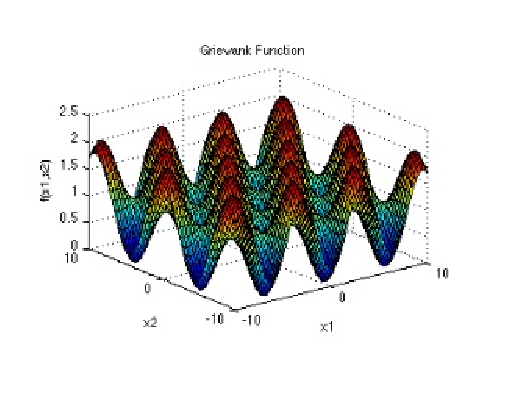
\includegraphics[width=0.8\linewidth]{eps/griewank.eps}
\caption{Griewank Function}
\label{fig:griewank}
\end{center}
\end{figure}
% \begin{figure}[t]
% 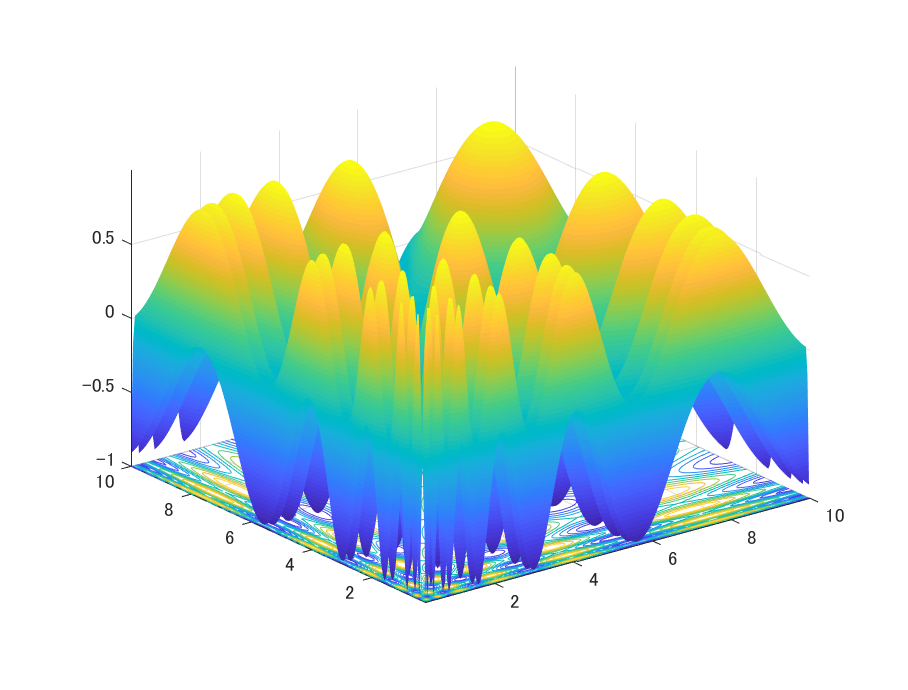
\includegraphics[width=0.8\linewidth]{eps/F7.eps}
% \caption{F7: Vincent Function}
% \label{fig:vincent}
% \end{figure}
% \begin{figure}[t]
% \includegraphics[width=0.8\linewidth]{eps/F9.eps}
% \caption{F9: Rastrigin Function}
% \label{fig:rastrigin}
% \end{figure}
\subsection{評価尺度}
提案手法の性能を検証するため,各解から最近傍個体間のユークリッド距離の総和を求める.評価式を以下に示す.MP(Max Peak)は全ての解数を表す.
\begin{equation}
dist = \sum_{j=1}^{MP} \sqrt{((解の座標)-(個体の座標))^2}
\end{equation}

\subsection{パラメータの設定}
個体数$N=50$とし,ラウドネス$A^0=1$,周波数$f_{max}=1$,${f_{min}=0}$,パルスレート$r^0 \in [0,1]$として設定した.また従来と同様,$\alpha= \gamma = 0.9$とし,世代数を1000,次元数$D=2$,実験の試行回数を30回と設定した.
\subsection{結果}
\begin{table}
\begin{center}
\caption{1000世代目における各手法のdistの平均値と標準偏差}
\label{tab}
\begin{tabular}{ccc}\hline
 & Mean & SD\\  \hline\hline
BA & 98.90122 & 22.23042 \\ 
NRBA & 10.05272 & 4.838307 \\ \hline
% NRBA10 & 15.15023 & 5.410486 \\ \hline
\end{tabular}
\end{center}
\end{table}
\begin{figure}[t]
\begin{center}
\includegraphics[width=0.8\linewidth]{eps/1000.eps}
\caption{1000世代目における個体の分布(NRBA)}
\label{fig:1000}
\end{center}
\end{figure}

表\ref{tab}は従来手法と提案手法の試行回数を30回実行した平均値とその標準偏差を示す.図\ref{fig:1000}は,平面を解空間の大きさを表し,色濃度は評価値を表す.

\subsection{考察}
表\ref{tab}の実験結果から,提案手法は複数の局所解と最適解に個体が到達しており,図\ref{fig:1000}からほぼ全ての解を捕捉できていると言える.
\section{おわりに}
本研究では最適解だけでなく,複数の局所解を同時に探索可能なBat Algorithmを提案した.従来手法と比較して最適解に陥らず,複数解を探索することができた.今後の課題としては,全ての解を探索すること,実問題への適用を考慮した個体数制限化での探索性能向上を目指す.
{\small
\begin{thebibliography}{*}
\bibitem{BA} Yang, X. S. “A Metaheuristic Bat-Inspired Algorithm”, {\it in: Nature Inspired Cooperative Strategies for Optimization (NISCO 2010) (Eds J.R. Gonzalez et al.)}, {\it Studies in Com-putational Intelligence}, Springer Berlin, 284, Springer, 65-74 (2010).
\bibitem{niche} D.Beasley, D.R. Bull, and R.R. Martin, "A sequantial niche technique for multimodal function optimization," {\it Evolutionary Computation}, vol. 1, no.2, pp. 101-125,1993.
\bibitem{cec2013} X. Li, A. Engelbrecht, and M. G. Epitropakis, "Benchmark Functions for CEC'2013 Special Session and Competition on Niching Methods for Multimodal Function Optimization", {\it Evol. Comput.} Mach. Learn. Group, RMIT University, Melbourne, VIC, Australia, Tech. Rep., 2013.
% \bibitem{crowdingDE} R. Thomsen, "Multimodal Optimization Using Crowding-Based Differential Evolution," {\it in Proc. IEEE Congr. Evol. Comput.,} pp.1382-1389, 2004.
\end{thebibliography}
}
\end{document}